\section{Models}
\begin{frame}{The Three Pillars of Learning}
    \centering
    % Scaled down to 85% to fit better
    \begin{tikzpicture}[
        scale=0.85, transform shape, 
        node distance=1.0cm and 0.3cm,
        box/.style={
            rectangle, rounded corners, draw=none, 
            text width=4.0cm, minimum height=1.8cm, 
            align=center, font=\small
        },
        title/.style={font=\bfseries\large},
        % Arrow style removed
    ]

        % --- Column 1: The Model (Active) ---
        \node[title, blue] (h_title) at (0,0) {1. The Model ($f_\theta$)};
        \node[box, fill=blue!10, below=0.2cm of h_title] (h_box) {
            \textbf{Design Choice:}\\
            ML (Linear, Kernel, Trees) \\ \& DL (MLP, CNN)
            \vspace{0.5em}
            
            \textbf{Depends on:}\\
            Data Type (Tabular, image) \\ \& Complexity
        };

        % --- Column 2: Loss Function (Dimmed) ---
        \node[title, red, opacity=0.4] (l_title) at (4.5,0) {2. Loss Function ($J$)};
        \node[box, fill=red!10, text=gray, opacity=0.5, below=0.2cm of l_title] (l_box) {
            \textbf{Design Choice:}\\
            MSE vs. Cross-Entropy
            \vspace{0.5em}
            
            \textbf{Depends on:}\\
            The Task\\
            (Regression vs. Classification)
        };

        % --- Column 3: Optimizer (Dimmed) ---
        \node[title, green!60!black, opacity=0.4] (o_title) at (9.0,0) {3. Optimizer};
        \node[box, fill=green!10, text=gray, opacity=0.5, below=0.2cm of o_title] (o_box) {
            \textbf{Design Choice:}\\
            Gradient Descent, Adam
            \vspace{0.5em}
            
            \textbf{Depends on:}\\
            Resources \& Scale\\
            \footnotesize{(Covered later in Deep Learning)}
        };

        % Arrows removed as requested

    \end{tikzpicture}

    \vspace{1em}

    \begin{block}{}
        We have covered the \textbf{Loss Functions}. \\
        Now, let's move on to the \textbf{Models} themselves ($f_\theta$).
    \end{block}
\end{frame}

% =================================================================
% INTRODUCTION TO MODELS (FIXED & OPTIMIZED)
% =================================================================
% =================================================================
% INTRODUCTION TO MODELS
% =================================================================
\section{Machine Learning Models}

\begin{frame}{What is a Model?}
    \begin{columns}[c]
        % Left: Concept
        \begin{column}{0.5\textwidth}
            \begin{tcolorbox}[colback=blue!5, title=\textbf{Definition}]
                A \textbf{Model} ($f_\theta$) is a simplified mathematical representation of reality.
                It maps inputs ($x$) to outputs ($\hat{y}$) using learned parameters ($\theta$).
            \end{tcolorbox}

            \vspace{1em}
            \textbf{The Goal:}
            Find the "best" function $f$ that minimizes the error between prediction $\hat{y}$ and reality $y$. 
            % \\ The relation between $x$ and $y$ could be very complex (non-linear) or very simple (linear). Choosing the correct model matter in getting best results and not over or under fit.
            

        \end{column}

        % Right: Vertical Visual Flow
        \begin{column}{0.5\textwidth}
            \centering
            % \resizebox{0.7\linewidth}{!}{ % Resize width to 70% of column to stay centered
            \begin{tikzpicture}[node distance=1.8cm, thick, auto]
                % 1. Input (Top)
                \node[draw, circle, fill=gray!10, minimum size=1cm] (x) {$x$};
                \node[left=0.5cm of x, font=\small, gray] {Input};

                % 2. Model (Middle)
                \node[draw, rectangle, fill=blue!10, minimum width=2.5cm, minimum height=1.5cm,
                      below of=x, align=center] (model) {\textbf{Model}\\$f_\theta(\cdot)$};
                \node[right=0.2cm of model, font=\small, align=left] {Parameters\\$\theta$};

                % 3. Prediction (Bottom)
                \node[draw, circle, fill=green!10, minimum size=1cm, below of=model] (yhat) {$\hat{y}$};
                \node[left=0.5cm of yhat, font=\small, green!60!black] {Pred};

                % 4. Reality (Next to Prediction)
                \node[draw, circle, fill=red!10, minimum size=1cm, right=2cm of yhat] (real) {$y$};
                \node[right=0.5cm of real, font=\small, red] {Truth};

                % Arrows
                \draw[->] (x) -- (model);
                \draw[->] (model) -- (yhat);
                \draw[<->, dashed, red] (yhat) -- node[above] {Error} (real);
            \end{tikzpicture}
            % }
        \end{column}
    \end{columns}
\end{frame}

\begin{frame}[allowframebreaks]{Models Complexity}
    
    % 1. Top Text (Full Width)
    The relationship between inputs $\bx$ and target $y$ varies wildly.
    Choosing the correct model family matters to avoid \textbf{Underfitting} (too simple) or \textbf{Overfitting} (too complex).

    \begin{itemize}
                \item \textbf{Simple:} Linear. \\ \textit{(e.g., House Size $\to$ Price)}
                \item \textbf{Complex:} Non-linear. \\ \textit{(e.g., Image Pixels $\to$ "Cat")}
            \end{itemize}

    \vspace{1em}

    % 2. Centered & Enlarged Plot
    \centering
    \resizebox{0.5\linewidth}{!}{ % Scales the plot to 70% of the slide width
    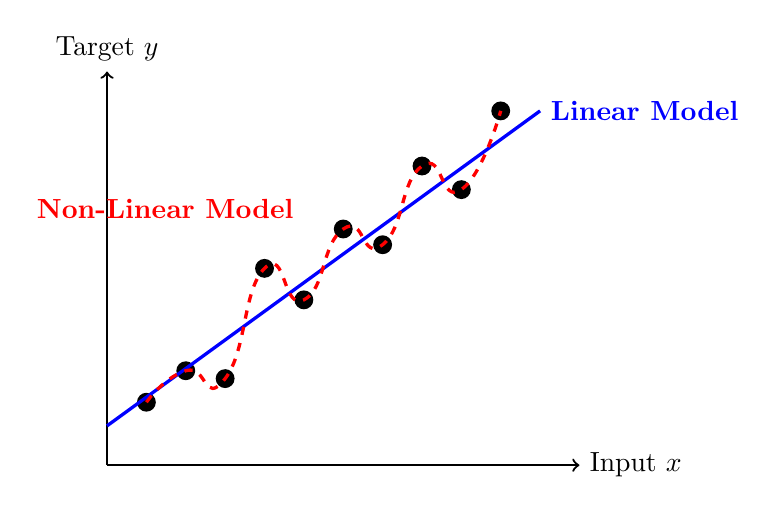
\begin{tikzpicture}[scale=1.0, thick]
        % Axes
        \draw[->] (0,0) -- (6,0) node[right] {Input $x$};
        \draw[->] (0,0) -- (0,5) node[above] {Target $y$};

        % Data Points
        \foreach \x/\y in {0.5/0.8, 1/1.2, 1.5/1.1, 2/2.5, 2.5/2.1, 3/3.0, 3.5/2.8, 4/3.8, 4.5/3.5, 5/4.5}
            \filldraw[black] (\x,\y) circle (3pt);

        % Linear Fit (Blue)
        \draw[blue, very thick] (0,0.5) -- (5.5,4.5) node[right] {\textbf{Linear Model}};

        % Non-Linear Fit (Red)
        \draw[red, very thick, dashed] plot [smooth, tension=1] coordinates {
            (0.5,0.8) (1,1.2) (1.5,1.1) (2,2.5) (2.5,2.1) (3,3.0) (3.5,2.8) (4,3.8) (4.5,3.5) (5,4.5)
        };
        \node[red, above left] at (2.5,3.0) {\textbf{Non-Linear Model}};
    \end{tikzpicture}
    }
\end{frame}

% --- SLIDE 2: TYPES OF MODELS (ML vs DL) ---
\begin{frame}{Machine Learning vs. Deep Learning}
    \centering
    \begin{columns}[T]
        % Left: Traditional ML
        \begin{column}{0.50\textwidth}
            \begin{tcolorbox}[colback=green!5, title=\textbf{1. Machine Learning (ML)}]
                Algorithms that parse data, learn patterns from it, and apply learned decisions.
            \end{tcolorbox}
            
            \vspace{0.5em}
            \textbf{Characteristics:}
            \begin{itemize}
                \item Best for \textbf{Structured Data} (Tables).
                \item Require \textbf{Feature Engineering}.
                \item Lightweight \& Interpretable (mostly).
            \end{itemize}
            
            \vspace{0.5em}
            \centering
            \textbf{Examples:}
            \footnotesize \textit{Linear Reg, SVM, Trees}
        \end{column}

        % Right: Deep Learning
        \begin{column}{0.50\textwidth}
            \begin{tcolorbox}[colback=blue!5, title=\textbf{2. Deep Learning (DL)}]
                A subset of Machine Learning based on artificial neural networks.
            \end{tcolorbox}
            
            \vspace{0.5em}
            \textbf{Characteristics:}
            \begin{itemize}
                \item Best for \textbf{Unstructured Data} (Images, Text, Audio).
                \item \textbf{Automated} Feature Extraction.
                \item Data \& Compute Hungry.
            \end{itemize}
            
            \vspace{0.5em}
            \centering
            \textbf{Examples:}
            \footnotesize \textit{MLPs, CNNs, Transformers}
        \end{column}
    \end{columns}
\end{frame}

% --- SLIDE 2: MACHINE LEARNING FOCUS ---
\begin{frame}{Machine Learning vs. Deep Learning}
    \centering
    \begin{columns}[T]
        % Left: Traditional ML
        \begin{column}{0.50\textwidth}
            \begin{tcolorbox}[colback=green!5, title=\textbf{1. Machine Learning (ML)}]
                Algorithms that parse data, learn patterns from it, and apply learned decisions.
            \end{tcolorbox}
            
            \vspace{0.5em}
            \textbf{Characteristics:}
            \begin{itemize}
                \item Best for \textbf{Structured Data} (Tables).
                \item Require \textbf{Feature Engineering}.
                \item Lightweight \& Interpretable (mostly).
            \end{itemize}
            
            \vspace{0.5em}
            \centering
            \textbf{Examples:}
            \footnotesize \textit{Linear Reg, SVM, Trees}
        \end{column}

        % Right: Transition Message
        \begin{column}{0.48\textwidth}
            \vspace{1.5cm} % Add some vertical space to center the text
            \centering
            \begin{tcolorbox}[colback=green!5, colframe=green!50, width=0.9\linewidth, arc=10pt]
                \centering
                \large
                \textbf{Let's start with \\ Machine Learning first.}
            \end{tcolorbox}
        \end{column}
    \end{columns}
\end{frame}

% =================================================================
% THE ML LANDSCAPE (FIXED SIZE)
% =================================================================

% --- SLIDE 4: THE COMPLEXITY SPECTRUM (UPDATED) ---
% =================================================================
% THE ML LANDSCAPE (ENLARGED & CENTERED)
% =================================================================

\subsection{Linear Models}

\begin{frame}{The ML Toolbox: Types of Models}
    \centering
    % Vertical space to center vertically
    \vspace*{\fill}
    \hspace*{-0.6cm}
    % Scaled up to fill the width of the slide
    \resizebox{1.1\linewidth}{!}{
    \begin{tikzpicture}[
        node distance=0.5cm,
        box/.style={
            scale=1.25, rectangle, draw=gray!40, fill=gray!5, 
            rounded corners, minimum width=2.8cm, minimum height=1.8cm, 
            align=center, font=\small
        },
        active/.style={
            draw=blue!80, fill=blue!10, line width=1.2pt
        },
        arrow/.style={-latex, thick, gray!60}
    ]
        % Top Node
        \node[font=\bfseries\Large] (root) at (0, 3) {Machine Learning Models ($f_\theta$)};

        % 1. Linear (Far Left)
        \node[box, active] (linear) at (-6, 0) {
            \textbf{1. Linear Models}\\
            % \vspace{0.3em}
            Linear Regression\\
            Logistic Regression        };

        % 2. Distance (Mid Left)
        \node[box] (distance) at (-2, 0) {
            \textbf{2. Distance-Based}\\
            KNN\\
            (Non-Parametric)        };

        % 3. Kernel (Mid Right)
        \node[box] (kernel) at (2, 0) {
            \textbf{3. Kernel-Based}\\
            SVM        };

        % 4. Trees (Far Right)
        \node[box] (trees) at (6, 0) {
            \textbf{4. Tree-Based}\\
            Decision Trees\\
            Random Forest\\
            Gradient Boosting        };

        % Connecting Arrows
        \draw[arrow] (root) -- (linear);
        \draw[arrow] (root) -- (distance);
        \draw[arrow] (root) -- (kernel);
        \draw[arrow] (root) -- (trees);

        % "Start Here" Annotation
        \node[blue, below=0.3cm of linear, font=\bfseries] {$\uparrow$ We Start Here!};

    \end{tikzpicture}
    }
    
    \vspace*{\fill}
\end{frame}


% =================================================================
% 1. LINEAR MODELS
% =================================================================
% =================================================================
% 1. LINEAR MODELS
% =================================================================
% =================================================================
% 1. LINEAR MODELS (Revised Section)
% =================================================================

% =================================================================
% 1. LINEAR MODELS
% =================================================================

% --- Slide 1: The Intuition (Scalar) ---
